\chapter{Experiments}
% This chapter presents the experiments. It is a crucial part of the thesis and has to dominate in the thesis. 
% The experiments and their analysis should be done in the way commonly accepted in the scientific community (eg. benchmark datasets, cross validation of elaborated results, reproducibility and replicability of tests etc).

\section{Methodology}
% \begin{itemize}
% \item description of methodology of experiments
% \item description of experimental framework (description of user interface of research applications – move to an appendix)
% \end{itemize}
One of the objectives of the thesis was to compare multiple shadow rendering methods both in a qualitative and quantitative ways. To achieve this a test renderer application was created, which implements the rendering techniques and allows a user to observe their results as well as profile the performance the program.

The tests were performed in a semi-controlled environment. Care was taken to avoid other processes interrupting and affecting the test results, but their impact could not be entirely eliminated in. Results of repeated tests at different moments in time or on different machines with the same hardware will differ, but that difference should not be large enough to impact the overall comparison results. 
% TODO: if you use two machines, mention it here.
The machine used for performing measurements had the following specification:
\begin{itemize}
    \item OS: Windows 10, 22H2
    \item CPU: AMD Ryzen 5 1600
    \item GPU: Nvidia GTX 1080, 8 GB VRAM
    \item RAM: 16 GB
\end{itemize}

\subsection{Created test application}
The test application allows the user to choose a rendering mode and observe the results in real time. It also allows to change the viewpoint and observe how the shadows behave in motion. Most rendering modes implement different shadow rendering techniques and some include debug views like wireframe mode or mesh colored by normals. The application is also instrumented with profiling commands which make it possible to connect to an external profiler and collect data in real time, as well as save and load existing profiling data.

As mentioned in section \ref{chapter:3_test_app}, the Tracy profiler open source library and tool was used to gather and visualize profiling data. For additional profiling and debugging RenderDoc, PIX and Nsight Graphics were used.

\section{Data sets}
The data sets consist of multiple scenes used for testing.
% TODO: describe the scenes.

\section{Results}
% \begin{itemize}
% \item presentation of results, analysis and wide discussion of elaborated results, conclusions
% \end{itemize}

The results of testing each implemented shadow rendering method are presented in the following sections. Each set of results is complemented by a description and discussion, highlighting possible causes and, if appropriate, possible fixes. The techniques might undergo different tests based on their characteristic.

\subsection{Planar shadow mapping}
% TODO: do I want to even test this?

\subsection{Basic shadow maps}
% TODO: test them with different scenes (complexity and scale), different shadow map resolutions, different render resolutions, different biases

\subsection{Filtered shadow maps}

\subsubsection{Hardware bilinear filtering}

\subsubsection{Percentage-closer filtering}

\subsubsection{PCF with bilinear filtering}

\subsubsection{Adaptive percentage-closer filtering}

% \begin{table}
% \centering
% \caption{A caption of a table is ABOVE it.}
% \label{id:tab:wyniki}
% \begin{tabular}{rrrrrrrr}
% \toprule
% 	         &                                     \multicolumn{7}{c}{method}                                      \\
% 	         \cmidrule{2-8}
% 	         &         &         &        \multicolumn{3}{c}{alg. 3}        & \multicolumn{2}{c}{alg. 4, $\gamma = 2$} \\
% 	         \cmidrule(r){4-6}\cmidrule(r){7-8}
% 	$\zeta$ &     alg. 1 &   alg. 2 & $\alpha= 1.5$ & $\alpha= 2$ & $\alpha= 3$ &   $\beta = 0.1$  &   $\beta = -0.1$ \\
% \midrule
% 	       0 &  8.3250 & 1.45305 &       7.5791 &    14.8517 &    20.0028 & 1.16396 &                       1.1365 \\
% 	       5 &  0.6111 & 2.27126 &       6.9952 &    13.8560 &    18.6064 & 1.18659 &                       1.1630 \\
% 	      10 & 11.6126 & 2.69218 &       6.2520 &    12.5202 &    16.8278 & 1.23180 &                       1.2045 \\
% 	      15 &  0.5665 & 2.95046 &       5.7753 &    11.4588 &    15.4837 & 1.25131 &                       1.2614 \\
% 	      20 & 15.8728 & 3.07225 &       5.3071 &    10.3935 &    13.8738 & 1.25307 &                       1.2217 \\
% 	      25 &  0.9791 & 3.19034 &       5.4575 &     9.9533 &    13.0721 & 1.27104 &                       1.2640 \\
% 	      30 &  2.0228 & 3.27474 &       5.7461 &     9.7164 &    12.2637 & 1.33404 &                       1.3209 \\
% 	      35 & 13.4210 & 3.36086 &       6.6735 &    10.0442 &    12.0270 & 1.35385 &                       1.3059 \\
% 	      40 & 13.2226 & 3.36420 &       7.7248 &    10.4495 &    12.0379 & 1.34919 &                       1.2768 \\
% 	      45 & 12.8445 & 3.47436 &       8.5539 &    10.8552 &    12.2773 & 1.42303 &                       1.4362 \\
% 	      50 & 12.9245 & 3.58228 &       9.2702 &    11.2183 &    12.3990 & 1.40922 &                       1.3724 \\
% \bottomrule
% \end{tabular}
% \end{table}  

% The table is here too \ref{id:tab:wyniki}

%%%%%%%%%%%%%%%%%%%%%
% FIGURE FROM FILE
%
% \begin{figure}
% \centering
% 
\includegraphics[width=0.5\textwidth]{./graf/politechnika_sl_logo_bw_pion_en.pdf}
% \caption{Caption of a figure is always below the figure.}
% \label{fig:label}
% \end{figure}

% Fig. \ref{fig:label} presents asdasd

% \begin{figure}
% 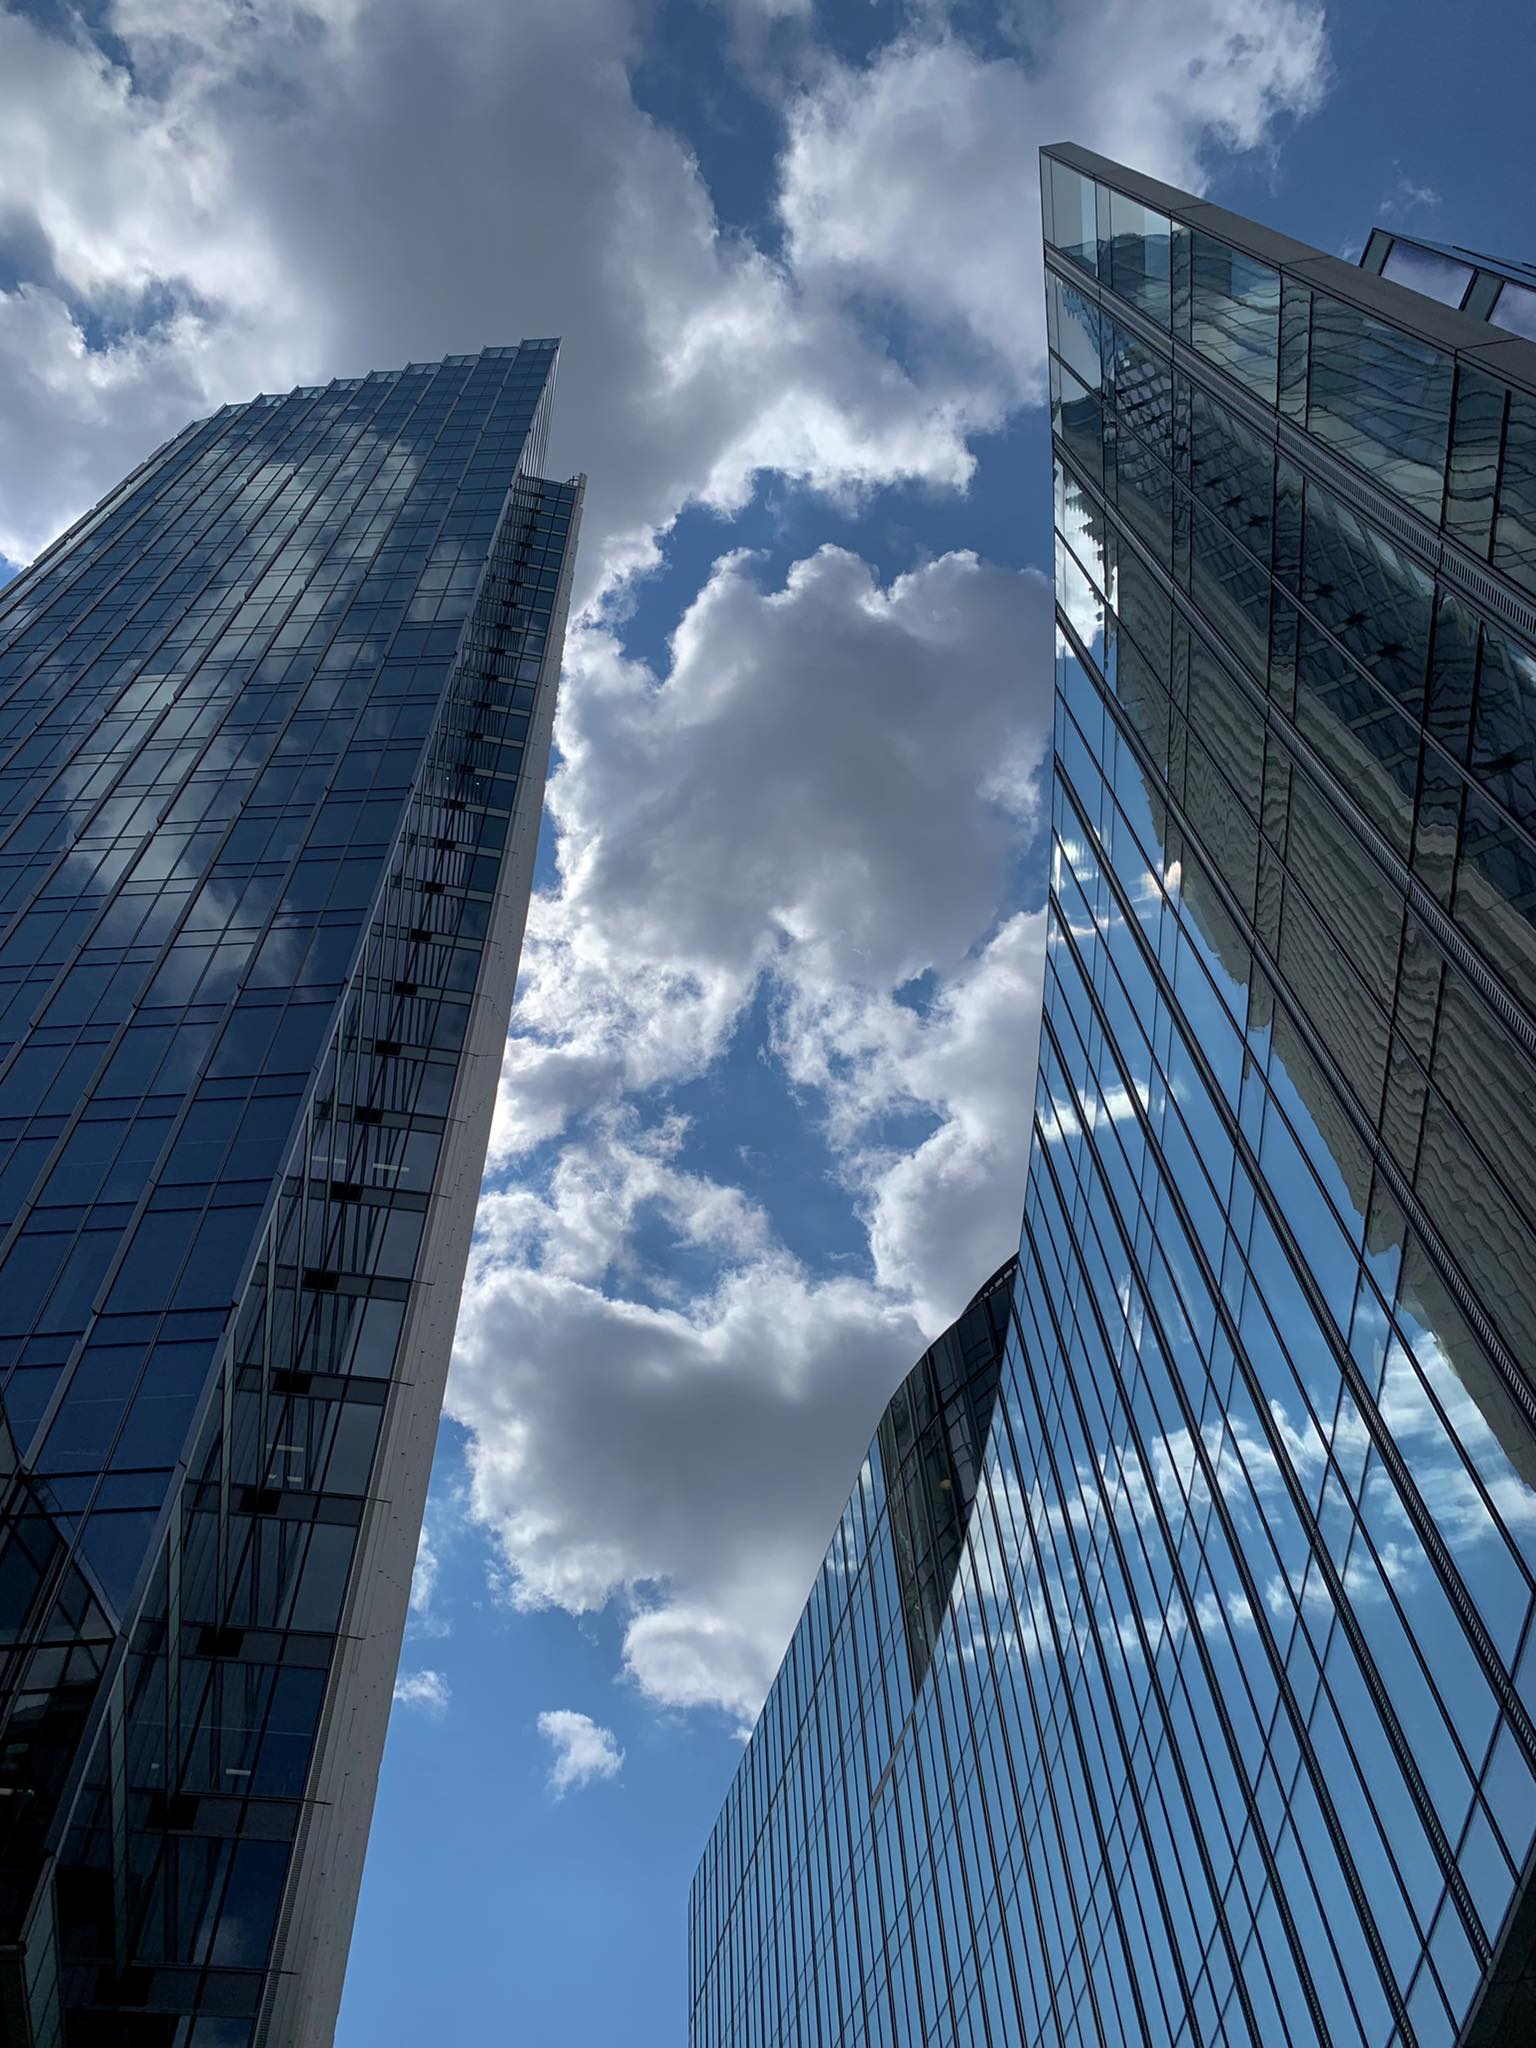
\includegraphics[width=0.5\textwidth]{./graf/test_image.jpg}
% \caption{Caption of a figure is always below the figure akakak.}
% \label{fig:duped_image3}
% \end{figure}

% some citation of the above \ref{fig:duped_image3}

%%%%%%%%%%%%%%%%%%%%%
%
%%%%%%%%%%%%%%%%%%%%
%% SUBFIGURES
%
% \begin{figure}
% \centering
% \begin{subfigure}{0.4\textwidth}
%    
\includegraphics[width=\textwidth]{./graf/politechnika_sl_logo_bw_pion_en.pdf}
%    \caption{Upper left figure.}
%    \label{fig:upper-left}
% \end{subfigure}
% \hfill
% \begin{subfigure}{0.4\textwidth}
%    
\includegraphics[width=\textwidth]{./graf/politechnika_sl_logo_bw_pion_en.pdf}
%    \caption{Upper right figure.}
%    \label{fig:upper-right}
% \end{subfigure}

% \begin{subfigure}{0.4\textwidth}
%    
\includegraphics[width=\textwidth]{./graf/politechnika_sl_logo_bw_pion_en.pdf}
%    \caption{Lower left figure.}
%    \label{fig:lower-left}
% \end{subfigure}
% \hfill
% \begin{subfigure}{0.4\textwidth}
%    
\includegraphics[width=\textwidth]{./graf/politechnika_sl_logo_bw_pion_en.pdf}
%    \caption{Lower right figure.}
%    \label{fig:lower-right}
% \end{subfigure}
       
% \caption{Common caption for all subfigures.}
% \label{fig:subfigures}
% \end{figure}
% Fig. \ref{fig:subfigures} presents very important information, eg. Fig. \ref{fig:upper-right} is an upper right subfigure.
%%%%%%%%%%%%%%%%%%%%%



% \begin{figure}
% \centering
% \begin{tikzpicture}
% \begin{axis}[
%    y tick label style={
%        /pgf/number format/.cd,
%            fixed,   % po zakomentowaniu os rzednych jest indeksowana wykladniczo
%            fixed zerofill, % 1.0 zamiast 1
%            precision=1,
%        /tikz/.cd
%    },
%    x tick label style={
%        /pgf/number format/.cd,
%            fixed,
%            fixed zerofill,
%            precision=2,
%        /tikz/.cd
%    }
% ]
% \addplot [domain=0.0:0.1] {rnd};
% \end{axis} 
% \end{tikzpicture}
% \caption{Figure caption is BELOW the figure.}
% \label{fig:3}
% \end{figure}

% \begin{figure}
% \centering
% 
\includegraphics[width=0.5\textwidth]{./graf/politechnika_sl_logo_bw_pion_en.pdf}
% \caption{Caption of a figure is always below the figure akakak.}
% \label{fig:3}
% \end{figure}

% some citation of the above \ref{fig:3}

% \begin{figure}
% \begin{lstlisting}
% if (_nClusters < 1)
% 	throw std::string ("unknown number of clusters");
% if (_nIterations < 1 and _epsilon < 0)
% 	throw std::string ("You should set a maximal number of iteration or minimal difference -- epsilon.");
% if (_nIterations > 0 and _epsilon > 0)
% 	throw std::string ("Both number of iterations and minimal epsilon set -- you should set either number of iterations or minimal epsilon.");
% \end{lstlisting}
% \caption{Example of pseudocode.}
% \end{figure}